% =============================================================================
% article_draft.tex — DRAFT, snn_separation
%
% Zakres: artykuł o NARZĘDZIU i MECHANIZMIE. Nie przesądza tezy pracy — ta decyzja
% jest otwarta (STATUS.md sek. 4.1); wyniki są raportowane jako demonstracje tego,
% co warsztat rozstrzyga. Wersja zwięzła z 2026-10-07.
%
% Kompilacja: pdflatex article_draft.tex (dwa przebiegi; bibliografia inline).
% Figury: article/figures/*.png — generuje make_article_figures.py.
% =============================================================================

\documentclass[11pt,a4paper]{article}

\usepackage[utf8]{inputenc}
\usepackage[T1]{fontenc}
\usepackage[english]{babel}
\usepackage{amsmath,amssymb}
\usepackage{graphicx}
\usepackage{booktabs}
\usepackage{siunitx}
\usepackage[margin=2.5cm]{geometry}
\usepackage[hidelinks]{hyperref}
\usepackage{xcolor}
\usepackage{caption}

\captionsetup{font=small,labelfont=bf}
\graphicspath{{figures/}}

\newcommand{\todo}[1]{\textcolor{red}{\textbf{[TODO: #1]}}}
\newcommand{\Kgc}{K_{\mathrm{GC}}}
\newcommand{\Wfsgc}{W_{\mathrm{FS}\to\mathrm{GC}}}

\title{\textbf{An interactive, data-constrained spiking model of the dentate
gyrus for studying pattern separation}}

\author{Jakub Caputa\thanks{\todo{affiliation, e-mail}} \and \todo{co-authors}}

\date{Draft --- \today}

\begin{document}
\maketitle

\begin{abstract}
\noindent
The dentate gyrus (DG) is thought to perform pattern separation: it turns similar
inputs into less similar outputs. The standard measure of this --- the drop in
correlation between output population vectors --- also rises whenever the network
simply fires less, so it is easy to mistake silence for separation. We present an
open spiking model of the DG microcircuit (granule cells, fast-spiking
interneurons, mossy cells) whose operating point is consistent with patch-clamp data,
together with two interfaces: a browser application in which an experimentalist
can change any biophysical parameter and see the effect immediately, and a
command-line layer that runs the same model on large parameter grids. Using it, we
show that apparent optima of separation move with the analysis threshold, that
phasic inhibition has no effect on separation once activity is held fixed, and that
the two most natural control codes bracket the circuit instead of providing a chance
level. The only circuit effect we see concerns regulation, not separation: with
mossy cells active the network can ignite, and phasic inhibition prevents it ---
but a confirmatory test on new seeds found ignition too rare at our current
weights to pass its pre-specified criterion.
\end{abstract}

% =============================================================================
\section{Introduction}
% =============================================================================

The DG receives overlapping activity patterns from the entorhinal cortex and is
thought to recode them into less overlapping granule cell patterns, so that CA3
can store them as distinct memories \cite{marr1971,treves1994,leutgeb2007}. Three
features are usually invoked: a large, sparsely active granule cell population;
strong feedforward and feedback inhibition from fast-spiking basket cells; and
an excitatory loop through hilar mossy cells whose net effect is debated.

Which of these carries the effect, and how much of each is needed, are
quantitative questions. Answering them needs a model that is constrained by data,
cheap enough to sweep, and transparent enough for experimentalists to question
directly. This paper describes such a model and the tools built around it
(Sections~\ref{sec:mechanism}--\ref{sec:app}), and the first experiments run with
it (Section~\ref{sec:experiments}). It does not yet argue for a single mechanistic
claim; open questions are listed in Section~\ref{sec:outlook}.

% =============================================================================
\section{Pattern separation and how it is measured}
\label{sec:mechanism}
% =============================================================================

We present two input patterns, measure their similarity $r_{in}$, record the
granule cell responses, and measure their similarity $r_{out}$. Here $r$ is the
mean pairwise Pearson correlation between population vectors. The circuit
separates the patterns when
\begin{equation}
  \mathrm{dec} \;=\; r_{in} - r_{out} \;>\; 0
  \label{eq:dec}
\end{equation}
(Figure~\ref{fig:concept}).

\begin{figure}[htbp]
  \centering
  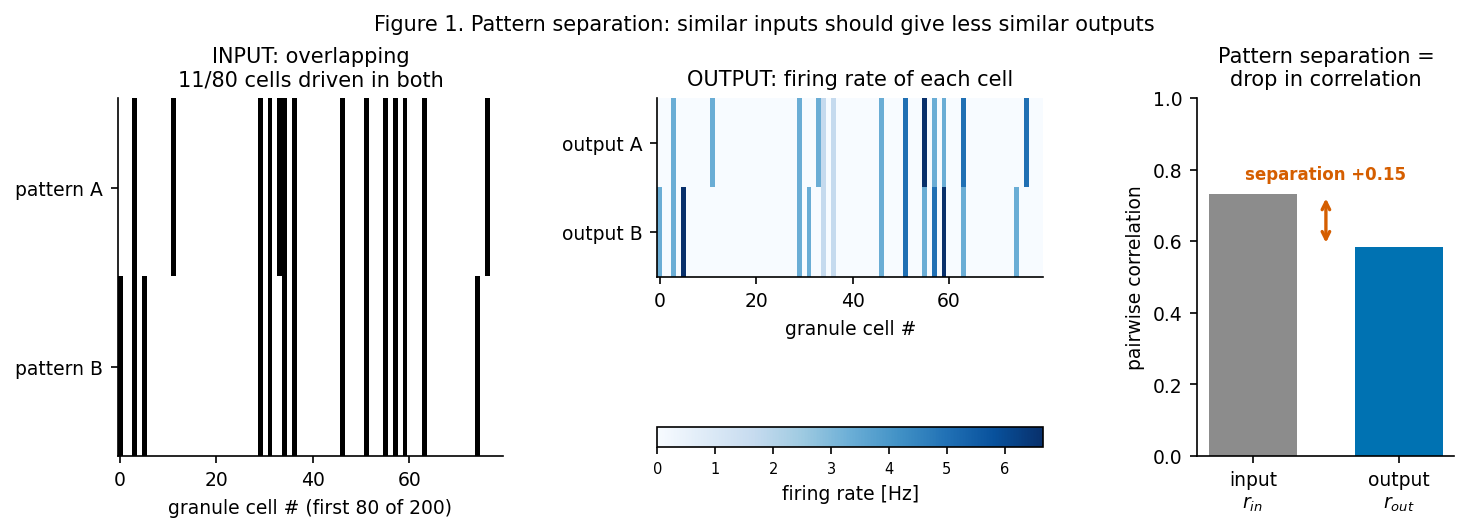
\includegraphics[width=\textwidth]{fig1-concept.png}
  \caption{\textbf{Pattern separation.} Two input patterns drive overlapping
  sets of granule cells (left); each cell fires at some rate (centre); output
  correlation is lower than input correlation, and the difference is
  $\mathrm{dec}$ (right). One run of the model at default parameters.}
  \label{fig:concept}
\end{figure}

\paragraph{The measurement trap.} The correlation between two nearly empty
vectors tends to zero. A network that stops firing therefore scores high on
Eq.~\eqref{eq:dec} while computing nothing. Any manipulation that lowers activity
--- including any increase in inhibition --- raises $\mathrm{dec}$ for reasons
unrelated to the circuit. Section~\ref{sec:experiments} is largely about getting
around this.

\paragraph{Two kinds of inhibition, three motifs.} The model separates
\emph{tonic} inhibition $\Kgc$, a constant hyperpolarising current that is always
on, from \emph{phasic} inhibition $\Wfsgc$, delivered by interneuron spikes. The
two are often lumped together; only the second belongs to a circuit motif. The
circuit decomposes into three motifs that can be switched off independently
(Figure~\ref{fig:circuit}): feedforward \textbf{FF} (PP\,$\to$\,FS\,$\to$\,GC),
feedback \textbf{FB} (GC\,$\to$\,FS\,$\to$\,GC), and the mossy cell loop
\textbf{MC} (GC\,$\to$\,HMC\,$\to$\,GC/FS).

\begin{figure}[htbp]
  \centering
  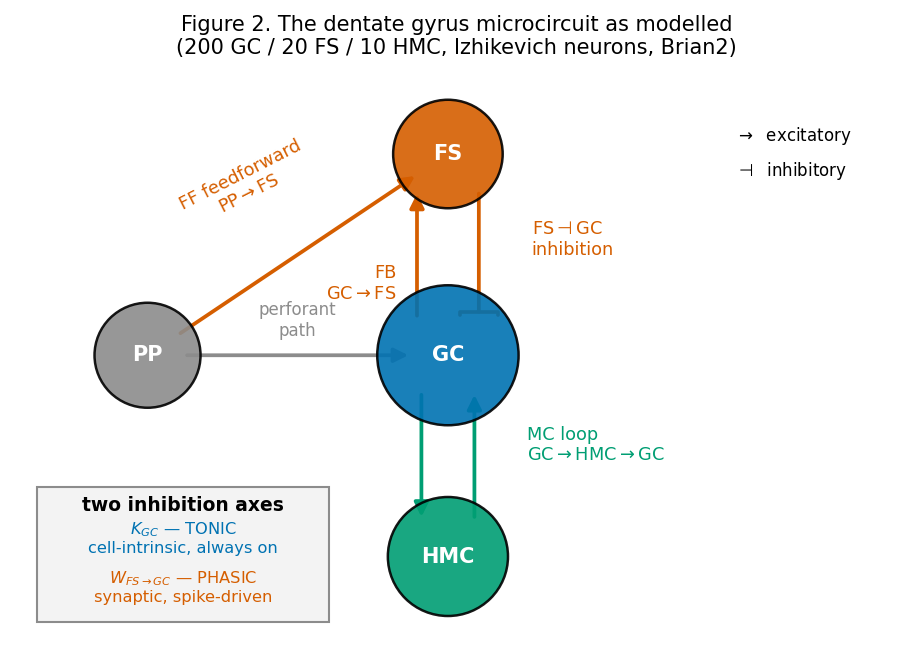
\includegraphics[width=0.75\textwidth]{fig2-circuit.png}
  \caption{\textbf{The modelled circuit.} Perforant path (PP) input drives
  granule cells (GC) and, in parallel, fast-spiking interneurons (FS); GC also
  drive FS; FS inhibit GC. Mossy cells (HMC) form an excitatory loop.}
  \label{fig:circuit}
\end{figure}

% =============================================================================
\section{Model}
\label{sec:model}
% =============================================================================

All cells are Izhikevich neurons \cite{izhikevich2003}, simulated in Brian2
\cite{stimberg2019}:
\begin{align}
  \frac{dv}{dt} &= 0.04\,v^2 + 5v + 140 - u + g_{ex} - g_{in} - K,
  \label{eq:izh_v}\\
  \frac{du}{dt} &= a\,(b\,v - u),
\end{align}
with reset $v \leftarrow c$, $u \leftarrow u + d$. Synaptic terms decay
exponentially ($\tau_{ex}=\SI{5}{\milli\second}$, $\tau_{in}=\SI{8}{\milli\second}$
for granule cells). Tonic inhibition is the term $K$, which enters the voltage
equation directly; this is what makes it separable from synaptic inhibition.
Parameters are in Table~\ref{tab:params}.

\begin{table}[htbp]
  \centering
  \small
  \caption{Default parameters. Weights are instantaneous post-synaptic
  depolarisation in mV.}
  \label{tab:params}
  \begin{tabular}{llll}
    \toprule
    & \textbf{GC} & \textbf{FS} & \textbf{HMC}\\
    \midrule
    Cells                      & 200 & 20 & 10 \\
    Izhikevich $a,b,c,d$       & 0.02,\,0.2,\,$-65$,\,6
                               & 0.10,\,0.2,\,$-65$,\,2
                               & 0.02,\,0.2,\,$-65$,\,4 \\
    $\tau_{ex}$ [ms]           & 5 & 3 & 5 \\
    Tonic inhibition $K$       & 10 & 5 & 10 \\
    \midrule
    \multicolumn{4}{l}{\textbf{Connection probability:}
      PP$\to$FS 0.40, GC$\to$FS 0.40, FS$\to$GC 0.50,
      GC$\to$HMC 0.25, HMC$\to$FS 0.40, HMC$\to$GC 0.40}\\
    \multicolumn{4}{l}{\textbf{Weights:}
      PP$\to$GC 4.0, PP$\to$FS 0.25, GC$\to$FS 10.0, FS$\to$GC 1.0,
      GC$\to$HMC 1.0, HMC$\to$FS 1.0, HMC$\to$GC 0.5}\\
    \multicolumn{4}{l}{\textbf{Simulation:}
      $dt=\SI{0.1}{\milli\second}$, $T=\SI{600}{\milli\second}$,
      PP delay \SI{4}{\milli\second}, other delays \SI{1}{\milli\second}}\\
    \bottomrule
  \end{tabular}
\end{table}

\paragraph{Input.} Each granule cell receives 40 perforant path fibres, firing at
\SI{10}{\hertz} for a driven cell and \SI{1}{\hertz} otherwise (\SI{400}{\hertz}
and \SI{40}{\hertz} in aggregate). The resulting steady-state drive is
\begin{equation}
  g_{ex} = r \cdot W \cdot \tau_{ex} = 400 \cdot 4 \cdot 0.005 = \SI{8}{\milli\volt}.
  \label{eq:gex}
\end{equation}
At \SI{600}{\hertz} granule cells would fire at \SI{16.6}{\hertz}, far denser
than in the DG.

\paragraph{Why the code is sparse.} For the Izhikevich neuron the threshold is a
fixed point of Eq.~\eqref{eq:izh_v}, available in closed form. The drive needed to
fire is
\begin{equation}
  G_{crit} = 4 + K
  \label{eq:gcrit}
\end{equation}
(confirmed by simulation to \SI{0.1}{\milli\volt}). At $\Kgc=10$ this is
\SI{14}{\milli\volt}, above the mean drive of an active granule cell,
$\SI{400}{\hertz}\times\SI{4}{\milli\volt}\times\SI{5}{\milli\second}
=\SI{8}{\milli\volt}$: granule cells fire only on fluctuations, which is why the
code is sparse (Figure~\ref{fig:opoint}a). The weight of \SI{4}{\milli\volt} is
not measured; it was chosen to give granule-cell rates of a few hertz, so panel~(a)
describes the regime rather than constraining it.

\paragraph{Data constraints.} The same parameter sets the resting potential, which
we compare with whole-cell recordings of Madar, Ewell \& Jones \cite{madar2019}
(BioStudies \texttt{S-BSST219}), read from the experimenters' annotations. After
removing duplicate records (72 records, 42 granule cells), the median resting
potential is $-76$\,mV (IQR $-81$ to $-70$). The model rests at $-78.7$\,mV at
$\Kgc=10$, inside that range (Figure~\ref{fig:opoint}b). The data constrain
$\Kgc$ to roughly 0--13.6 rather than to a single value. Note that matching low
activity levels (2--5\%) in the experiments below requires $\Kgc\approx14$--17,
slightly more hyperpolarised than three quarters of the recorded cells.

\begin{figure}[htbp]
  \centering
  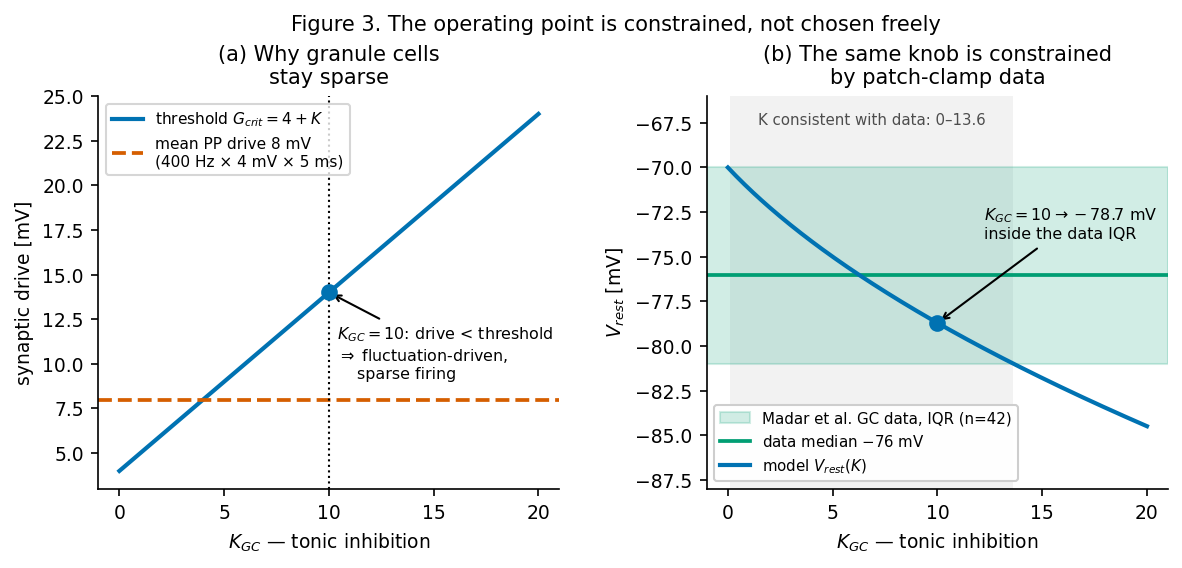
\includegraphics[width=\textwidth]{fig3-operating-point.png}
  \caption{\textbf{The operating point is consistent with data.} (a) Threshold
  $G_{crit}=4+K$ and the mean perforant path drive (\SI{8}{\milli\volt}); at
  $\Kgc=10$ the drive is below threshold. (b) The model's resting potential
  against patch-clamp data from 42 granule cells; grey band: values of $\Kgc$
  consistent with the interquartile range.}
  \label{fig:opoint}
\end{figure}

\todo{Methods: membrane time constant from the data is
$\approx\SI{3}{\milli\second}$ for granule cells, not 10--50\,ms. Irrelevant for
the Izhikevich model, but the definition (input vs membrane resistance) needs
checking.}

% =============================================================================
\section{The application}
\label{sec:app}
% =============================================================================

Both interfaces call one implementation of the circuit. An earlier version in
which the two had drifted apart produced results that did not match the tool.

\paragraph{Interactive tool.} \texttt{interactive\_dg.py} is a browser
application (Streamlit) for experimental collaborators. Every parameter in
Table~\ref{tab:params} is a slider, and the tool shows live: membrane traces for
two input patterns; input and output correlation matrices side by side, i.e.\
Eq.~\eqref{eq:dec} made visible; a circuit diagram with connection widths
proportional to current flow; a \emph{voltage budget} of what excites and what
inhibits granule cells; and the spike probability under the stimulation protocol
of Madar et al., for comparison with the experiment. A question such as ``what
happens if basket cell inhibition is halved?'' can be answered in the browser,
without reading code.

\paragraph{Command-line layer.} \texttt{experiments/dg\_core/} holds the same
circuit together with pattern generators, metrics, calibration routines and
control codes. Experiment scripts split parameter grids into shards for a SLURM
cluster; the grids below run in minutes on 16 cores.

\paragraph{Calibration instead of tuning.} Target quantities are hit by bisection
rather than by hand. In particular, bisection on $\Kgc$ sets the fraction of
active granule cells to a requested value. This turns activity from an outcome
into a controlled variable, which Section~\ref{sec:matched} relies on.

\paragraph{Reproducibility.} Regression tests (17) check that default behaviour
stays bit-for-bit identical as features are added.
\todo{container, configuration files, Zenodo deposit}

% =============================================================================
\section{Experiments so far}
\label{sec:experiments}
% =============================================================================

Figure~\ref{fig:findings} summarises the experiments.

\begin{figure}[htbp]
  \centering
  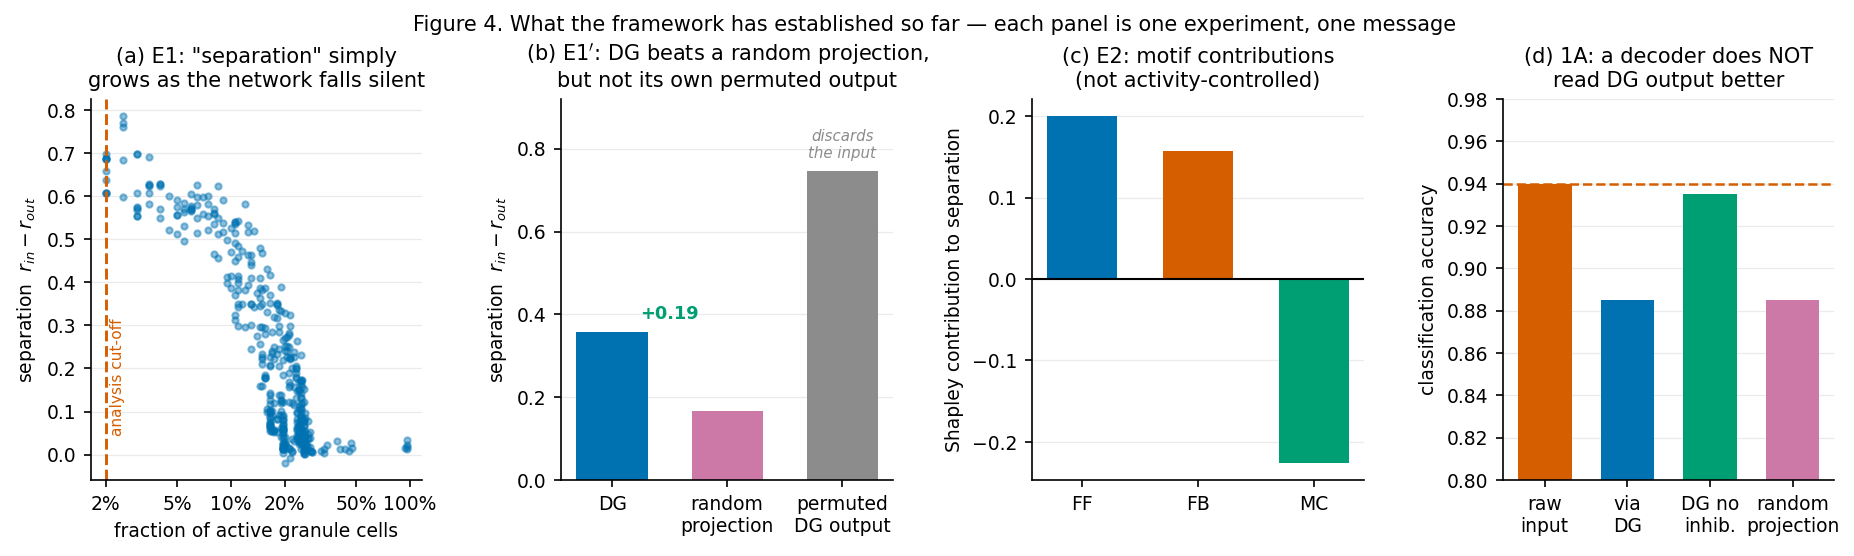
\includegraphics[width=\textwidth]{fig4-findings.png}
  \caption{\textbf{Experiments to date.} (a) Separation rises as the network
  falls silent; the apparent optimum sits at the analysis cut-off.
  (b) At fixed activity, DG separates more than the random-projection null but
  less than its own permuted output (both defined in
  Section~\ref{sec:nulls}). (c) Shapley contributions of the three motifs; not
  controlled for activity (Section~\ref{sec:e2}). (d) A linear classifier reads
  the raw input better than DG output.}
  \label{fig:findings}
\end{figure}

\subsection{E1: no optimum of separation}

We swept $\Kgc$ and $\Wfsgc$ over a $10\times9$ grid with five seeds (450 points)
and asked whether separation peaks at intermediate activity. It does not:
separation rises monotonically as activity falls (Figure~\ref{fig:findings}a).
Because points below an activity cut-off are discarded --- a standard guard
against the trap of Section~\ref{sec:mechanism} --- the maximum lands just above
the cut-off and moves with it: cut-offs of 2, 5, 10 and 20\% active cells put the
maximum at 2.5, 6.5, 12 and 20\%. A maximum that follows the analyst's threshold
belongs to the analysis, not the circuit.

\subsection{E1$'$: holding activity fixed}
\label{sec:matched}

To remove the confound we set activity by bisection on $\Kgc$ (6 levels, 2--30\%
active cells) and then varied phasic inhibition $\Wfsgc$ from 0 to 5 (9 values,
3 input sparsities, 5 seeds; 733 of 810 points reached the requested activity).
Raising $\Wfsgc$ therefore replaces tonic with phasic inhibition at constant
activity.

At fixed activity, phasic inhibition does not change separation. Per-level slopes
are slightly negative and none survives correction for six comparisons (smallest
$p=0.033$ against a threshold of $0.008$); the pooled slope is $-0.003$
($p=0.60$). The effect of inhibition seen in E1 was an effect of activity.

\subsection{Choosing a control code}
\label{sec:nulls}

To credit the circuit with separation, it must beat a code of the same sparsity
that has no circuit --- a \emph{null}. We used two:

\begin{description}
  \item[Permutation null] (``permuted DG output''): the DG output rates,
        shuffled across cells separately for each pattern. Same rates, but no
        link between pattern and cell.
  \item[Random-projection null] (``random projection''): the input pattern passed
        through a random Gaussian matrix, keeping as many active units as DG has.
        Same sparsity, still input-driven, but no circuit.
\end{description}

Neither gives a chance level (Figure~\ref{fig:nulls}a). Shuffling destroys all
information about the stimulus, so the permutation null's output correlation is
zero and its score equals the input correlation:
\begin{equation}
  \mathrm{dec}_{\mathrm{perm}} \approx r_{in}
  \;\Longrightarrow\;
  \mathrm{dec} - \mathrm{dec}_{\mathrm{perm}} = -\,r_{out}
  \label{eq:degenerate}
\end{equation}
(measured: $0.5687$ against $r_{in}=0.5682$). The ``excess'' over this null is
just $-r_{out}$. It is a ceiling that only a code that ignores the stimulus can
reach. A random projection, by contrast, preserves inner products, so it barely
decorrelates. At $r_{in}=0.748$, output correlation is $0.001$ for the
permutation null, $0.580$ for the random projection and $0.390$ for DG: the two
nulls bracket the circuit rather than benchmark it.

DG beats the random projection by $+0.19$, but most of this margin does not come
from inhibition. With all inhibitory motifs removed, the circuit already achieves
$+0.094$ of the full circuit's $+0.152$ (Figure~\ref{fig:nulls}b). About 60\% of
the advantage is the spiking threshold itself.

\begin{figure}[htbp]
  \centering
  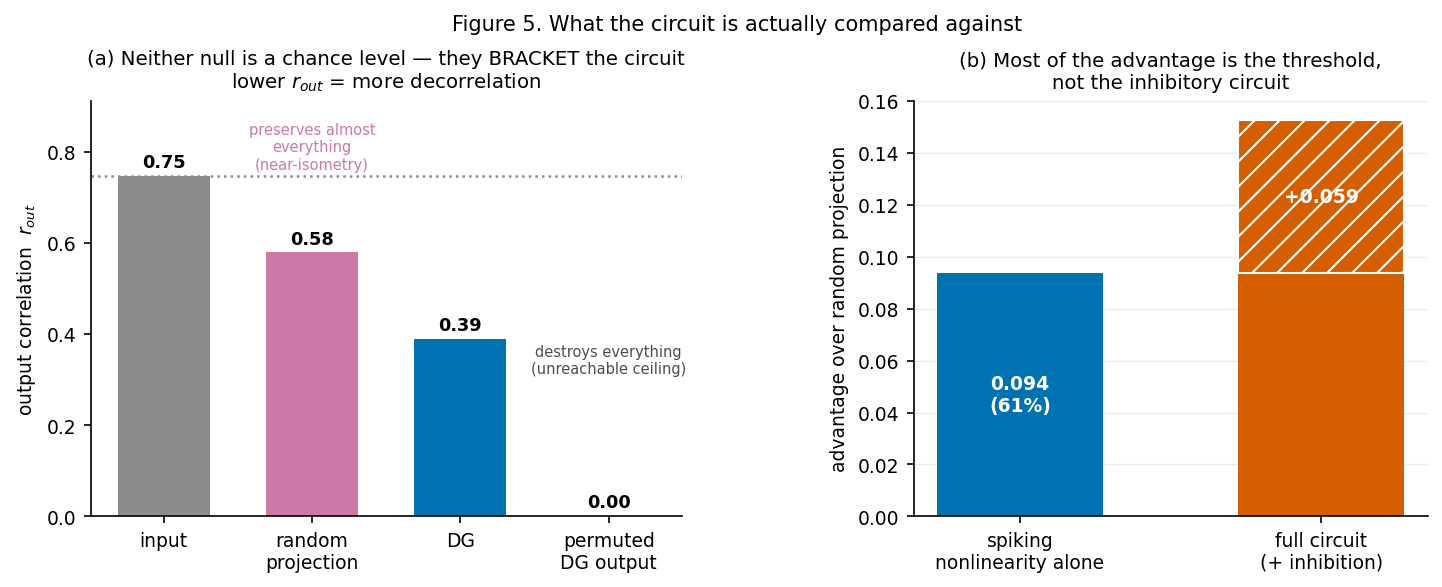
\includegraphics[width=\textwidth]{fig5-nulls.png}
  \caption{\textbf{The two nulls bracket the circuit.} (a) Output correlation
  for the raw input, the random-projection null, DG, and the permutation null.
  (b) DG's advantage over the random projection, with and without inhibition.}
  \label{fig:nulls}
\end{figure}

\subsection{E2: attributing separation to motifs}
\label{sec:e2}

With three motifs that can be removed independently, the contribution of each is
a Shapley value over the $2^3$ lesion combinations. At the canonical drive (36
input conditions, 5 seeds) the raw values are FF $+0.20$, FB $+0.16$ and mossy
cells $-0.23$, with strong positive interactions between mossy cells and either
inhibitory motif ($+0.21$ to $+0.22$; Figure~\ref{fig:findings}c).

These values are \emph{not} controlled for activity, and activity explains most of
them. Lesions change the fraction of active granule cells from 13\% to 94\%, and
across lesion combinations separation correlates with activity at $r=-0.97$. With
both inhibitory motifs removed, mossy cells drive 94\% of granule cells to fire
--- an ignition state that the inhibitory motifs prevent. The ``conditional'' role of mossy cells is
therefore primarily about keeping activity in check. Subtracting the
random-projection null, which does depend on activity, shrinks the contributions
by 15--27\% (mossy cells $-0.16$) but does not remove them. At half the drive all
contributions are several times smaller (mossy cells $-0.06$). Section~\ref{sec:wide} repeats the test with activity held fixed.

\subsection{E1$''$: a wider activity-matched sweep}
\label{sec:wide}

E1$'$ held three things fixed that might matter: input similarity
($r_{in}=0.75$), mossy cells (silent at default weights) and the measure (rate
correlation over \SI{600}{\milli\second}, blind to timing). E1$''$ varied all
three: input similarity 0.5--0.95, mossy cells silent or active, phasic
inhibition up to 12, at four activity levels (2--20\%) with five seeds (1280
points, 1267 tuned). It added a timing measure: how much more a pattern's response
resembles a repeat of itself than another pattern's response, in \SI{20}{\milli\second}
bins. Comparing against a repeat cancels Poisson noise, which would otherwise
lower the correlation by itself.

The analysis criterion was fixed before the run: a dependency on phasic inhibition
counts only if the slope is significant after Bonferroni correction over all tests
(40 tests, $p<1.25\times10^{-3}$) and is confirmed, with the same sign, at an
adjacent input similarity. \textbf{No dependency met it}, for separation or for
timing.

One pattern came close: with mossy cells active and 20\% of cells active,
separation dropped sharply between $\Wfsgc=0$ and $2$. The cause was not
separation. For some input patterns the network \emph{ignited} --- nearly all
granule cells fired --- while bisection, which tunes activity on a single pattern,
kept the tuned pattern at its target. (An earlier version of this analysis divided
the mean rate over all patterns by the active fraction of the tuned pattern and
reported this as cells firing at about \SI{280}{\hertz}; that measure mixed
patterns and is withdrawn.)

\paragraph{Confirmatory test (E1$'''$).} We then tested ignition directly, on new
seeds, with the strength of the mossy cell loop as an axis ($\lambda=0$: mossy
cells silent; $\lambda=1$: the weights of E1$''$; also $0.5$, $0.75$, $1.5$), at
fixed activity (1050 runs) and, separately, without matching activity (360 runs).
The criterion, fixed in code before the run, was that ignition is significantly
more frequent at $\Wfsgc=0$ than at $\Wfsgc=2$ for $\lambda=1$ and $1.5$.
\textbf{It was not met}: at $\lambda=1$ ignition occurred in 2 of 20 runs at
$\Wfsgc=0$ and none at $\Wfsgc=2$ ($p=0.24$); at $\lambda=1.5$, 4 of 20 vs none
($p=0.053$, threshold $0.025$). Exploratory regularities nevertheless hold across
all loop strengths (Figure~\ref{fig:runaway}): no ignition ever without mossy
cells (0 of 210 runs), none at $\Wfsgc\geq3$, and a frequency that grows with
loop strength (up to 40\% at $\lambda=1.5$). Without activity matching, at tonic
inhibition consistent with the patch-clamp data, removing phasic inhibition let
100\% of granule cells fire. Whether ignition is realistic therefore depends on
the strength of the mossy cell to granule cell pathway, which we have not yet
anchored in data.

\begin{figure}[htbp]
  \centering
  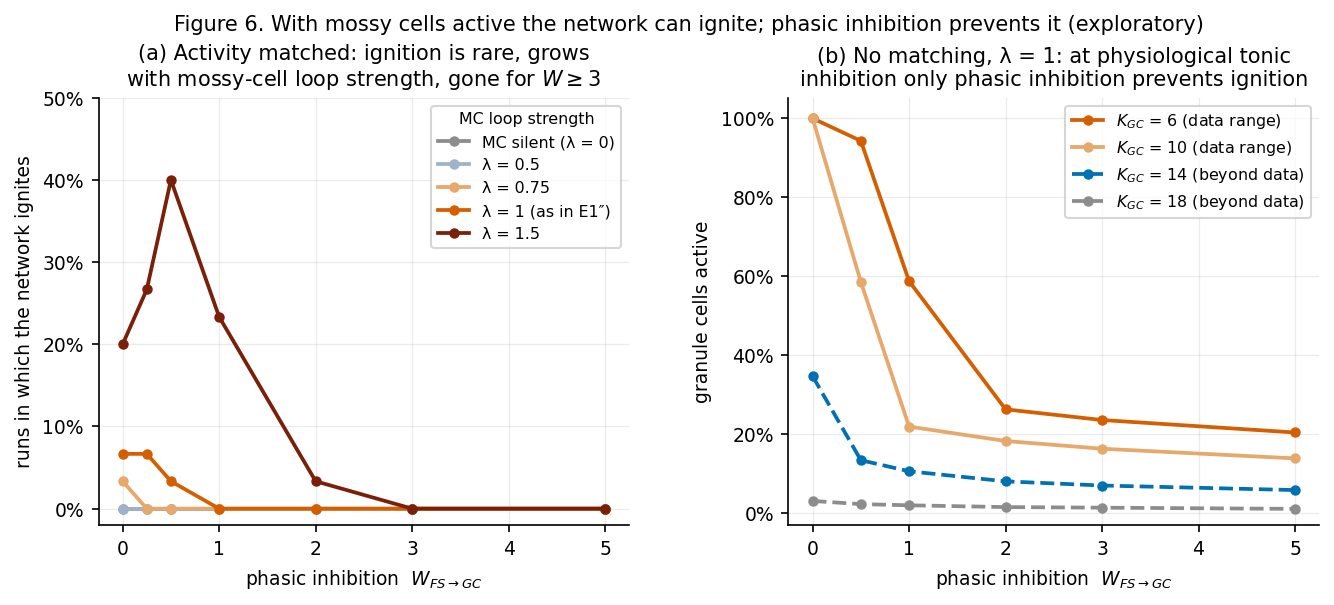
\includegraphics[width=\textwidth]{fig6-runaway.png}
  \caption{\textbf{With mossy cells active the network can ignite (exploratory).}
  (a) Activity held fixed: fraction of runs in which one input pattern drives
  nearly all granule cells, against phasic inhibition, for five strengths of the
  mossy cell loop. (b) No activity matching, $\lambda=1$: fraction of active
  granule cells for four levels of tonic inhibition; solid lines lie within the
  range consistent with the data.}
  \label{fig:runaway}
\end{figure}

\subsection{1A: does a downstream reader benefit?}

A linear classifier, which does not use correlation at all, reads pattern
identity from the raw input with accuracy $0.940$, from DG output with $0.885$,
from DG without inhibition with $0.935$, and from a random projection of equal
sparsity with $0.885$ (Figure~\ref{fig:findings}d). DG does not help the reader.

% =============================================================================
\section{Summary and open questions}
\label{sec:outlook}
% =============================================================================

\paragraph{Methodological lessons.} First, a drop in correlation is not evidence
of pattern separation unless activity is controlled: in our grids the confound is
larger than the effect, and discarding silent points only moves the apparent
optimum to the cut-off. Second, the obvious control --- shuffling the output ---
is degenerate (Eq.~\eqref{eq:degenerate}). A useful control must keep the
sparsity \emph{and} stay driven by the input; even then, a random projection is a
low bar. We used the degenerate control ourselves before noticing.

\paragraph{Results.} In this model, phasic inhibition has no effect on separation
at fixed activity, across input similarities and with or without mossy cells;
DG's advantage over the random projection comes mostly from the spiking threshold;
and DG does not help a linear reader. The motif attribution is dominated by
activity. What the circuit visibly does is regulate activity: with recurrent
excitation present, the network can ignite and phasic inhibition prevents it, but
how often this happens depends on a mossy cell weight we have not anchored in data.

\paragraph{Next steps.}
\begin{itemize}
  \item Anchoring the mossy cell to granule cell strength in data, which decides
        whether network ignition is a realistic regime of the model.
  \item Using the stimulation protocols of Madar et al.\ as model input.
  \item Since activity, not separation, is what the circuit visibly controls:
        progressive mossy cell loss as a model of temporal lobe epilepsy, and
        homeostatic regulation of the operating point.
  \item Separation grows with network size ($+0.149 \to +0.296$ for 200 $\to$ 800
        granule cells in preliminary runs); to be re-measured at fixed activity.
\end{itemize}

% =============================================================================
\section*{Code and data availability}
% =============================================================================

Model, application and experiment scripts: \todo{URL, DOI; BSD-3-Clause planned}.
Recordings: \cite{madar2019}, BioStudies \texttt{S-BSST219}; not redistributed.

\section*{Acknowledgements}
\todo{funding; PLGrid/ACK Cyfronet AGH computational grant; collaborators}

% =============================================================================
\begin{thebibliography}{9}
\small

\bibitem{marr1971} Marr, D. (1971). Simple memory: a theory for archicortex.
\emph{Phil. Trans. R. Soc. Lond. B} 262, 23--81.

\bibitem{treves1994} Treves, A. \& Rolls, E. T. (1994). Computational analysis
of the role of the hippocampus in memory. \emph{Hippocampus} 4, 374--391.

\bibitem{leutgeb2007} Leutgeb, J. K., Leutgeb, S., Moser, M.-B. \& Moser, E. I.
(2007). Pattern separation in the dentate gyrus and CA3 of the hippocampus.
\emph{Science} 315, 961--966.

\bibitem{izhikevich2003} Izhikevich, E. M. (2003). Simple model of spiking
neurons. \emph{IEEE Trans. Neural Netw.} 14, 1569--1572.

\bibitem{madar2019} Madar, A. D., Ewell, L. A. \& Jones, M. V. (2019).
Pattern separation of spiketrains in hippocampal neurons.
\emph{PLOS Computational Biology}. Data: BioStudies \texttt{S-BSST219}.

\bibitem{stimberg2019} Stimberg, M., Brette, R. \& Goodman, D. F. M. (2019).
Brian 2, an intuitive and efficient neural simulator. \emph{eLife} 8, e47314.

\todo{add: tonic GABA in DG; mossy cell function; sparse coding in DG; Shapley
attribution in neuroscience}
\end{thebibliography}

\end{document}
